\documentclass[man,floatsintext]{apa6}
%\usepackage[nodoi]{apacite}
\usepackage[natbibapa]{apacite} 
\bibliographystyle{apacite}
\usepackage{graphicx, subcaption}
\usepackage{amsmath}
\usepackage[american]{babel}
\usepackage[section]{placeins}
\usepackage[doublespacing]{setspace}
\usepackage{pslatex}
%\usepackage{cite} 
\usepackage{multirow}
\usepackage{url}
\usepackage{color,soul}
%\usepackage{csquotes}


\title{Observing and Modeling Developing Knowledge and Uncertainty during Cross-situational Word Learning}

\author{George Kachergis$^{1}$ and Chen Yu$^{2}$} 

\affiliation{
 $^{1}$Department of Artificial Intelligence \\
  Donders Institute for Brain, Cognition, and Behavior \\
  Radboud University \\
  6525 HR Nijmegen, the Netherlands \\
  
  $^{2}$Psychological \& Brain Sciences \\
   Indiana University \\
   Bloomington, Indiana 47408 
}

\shorttitle{Modeling Developing Cross-situational Knowledge}
\leftheader{Kachergis \& Yu}

\abstract{Being able to learn word meanings across multiple scenes consisting of multiple words and referents (i.e., cross-situationally) is thought to be important for language acquisition. The ability has been studied in infants, children, and adults, and yet there is much debate about the basic storage and retrieval mechanisms that operate during cross-situational word learning. It has been difficult to uncover the learning mechanics in part because the standard experimental paradigm, which presents a few words and objects on each of a series of training trials, measures learning only at the end of training, after several occurrences of each word-object pair. Diverse models are able to match the final level of performance of the standard paradigm, while the rich history and context of the learning trajectories remain obscured. This study examines accuracy and uncertainty over time in a version of the cross-situational learning task in which words are tested throughout training, as well as in a final test. With similar levels of performance to the standard task, we examine how well the online response trajectories match recent hypothesis- and association-based computational models of word learning.}

\keywords{Cross-situational word learning, language acquisition, statistical learning, memory-guided attention}
\authornote{This work was in part funded by National Institute of Health Grants R01HD056029 and R01HD074601.


Please address correspondence to George Kachergis, Radboud University, Montessorilaan 3, 6525 HR Nijmegen, the Netherlands 10003. Email: g.kachergis@donders.ru.nl}

\begin{document}
\maketitle

\section{Introduction}


Language acquisition, a problem that we all solve as infants and yet one that continues to baffle robots (not to mention researchers), may be better viewed--if perhaps not solved--as a constellation of problems including segmenting the continuous speech streams we hear into discrete words \cite[e.g.][]{Saffran:1996vn}, learning syntax \cite[e.g.][]{Reber:1967}, and learning the referential intent (i.e., meanings--concrete or abstract) of words \cite[e.g.,][]{Yu:2007}. These various subproblems of language acquisition have in recent decades been investigated under the umbrella of statistical learning. As they inquire whether and how people extract regularities from their environment, studies of statistical learning often overlap in assumptions and interpretation with implicit learning studies \citep{Perruchet:2006}. The present study focuses on a particular problem in language acquisition: that of learning word-object mappings from a series of ambiguous situations containing multiple words and objects, a process referred to as cross-situational word learning \citep{Gleitman:1990}. In a typical cross-situational learning study of adults \citep{Yu:2007}, a few unusual objects are presented on each trial and are then named in a random order. Thus, from a single trial participants can only guess which word refers to which object. However, since pairs occur on multiple trials spread across training, and appear with different concurrent pairs, people can learn some of the intended word-object pairings. As each word is heard on a trial, presumably interacting memory and learning processes drive attention to strengthen particular associations (or store particular hypotheses, in another view). 

Previous research has shown young children are capable of learning cross-situationally \citep{Suanda:2014}, and in adults examined the impact of factors such as frequency and contextual diversity \citep{Kachergis:2016} and spacing of stimuli \citep{Kachergis:2009tc}, as well as detailed analyses showing the impact of varied study and test contexts \citep{Suanda:2012,Vouloumanos:2008te}. A drawback of most extant studies is that learning is typically only measured at one point in time (i.e., at a final test), leaving the timecourse of learning unelaborated. Such knowledge would be quite informative for distinguishing different mechanistic accounts, as computational models with distinct assumptions can often mimic each other at a single point in time \citep{Yu:2012hyp}. Moreover, it is of interest in human-robot interaction, where investigations of incremental word learning in robots are aimed at producing systems that adapt in order to communicate more effectively \citep{SeabraLopes:2007}. Achieving a better understanding of statistical language learning in people may therefore also allow us to create algorithms allowing robots to learn and communicate more like humans \citep{Lyon:2012}.
How are we to reveal the interactions of learning, memory, and attention mechanisms during training that produce differences in final learning outcomes?
The present study compares a standard passive cross-situational training procedure--with four words-object pairs per trial--to a response procedure, in which participants must respond to each word on a training trial by clicking on one of the objects or a ``Don't Know'' button. Although this response procedure alters the task, it also offers a glimpse into the ongoing learning during training that can grant greater insight into the mechanisms at play.

Consider the possible progress of learning on a couple of training trials with 3 words and objects, e.g. those shown in Figure~\ref{fig:intro_example}. Suppose participants hear novel words ${bosa, manu, plimbi}$ while viewing objects ${o_1, o_2, o_3}$ on trial $t$. A few trials later ($t+3$), hearing ${manu, stigson, bosa}$ while seeing ${o_3, o_2, o_4}$, what might the participant learn? There are two basic perspectives on how people learn word-object mappings. In the hypothesis-testing view, learners store only a single hypothesized referent for each word--randomly at first, discarding the hypothesis only if it is disconfirmed \citep{Medina:2011,Trueswell:2013}. This perspective typically views language acquisition as an inference problem to be solved by applying logical constraints \citep{Siskind:1996}. In this view, a learner may have stored $bosa-o_1$, $bosa-o_2$, or $bosa-o_3$--but not more than one of these. Moreover, if $bosa-o_1$ was stored, then $o_1$ could not be stored as the referent for any other word on the trial--a strict mutual exclusivity (ME) constraint. Infants and adults are known to show a bias for learning mutually exclusive word-object mappings, although adults will adaptively relax the bias when given evidence of non-ME pairings \citep{Kachergis:2012gi}. On the latter trial, a hypothesis-tester would throw out any hypotheses inconsistent with the current data (e.g., $manu-o_1$ would be thrown out). A hypothesis-tester would consider the second trial to be confirming evidence of $bosa-o_3$ and $manu-o_2$ -- or vice-versa, depending on which hypotheses happened to be made on the first trial. Such a learner would \textit{not} know that they should still be uncertain of which mapping is correct.

\begin{figure}[h]
  \centering
  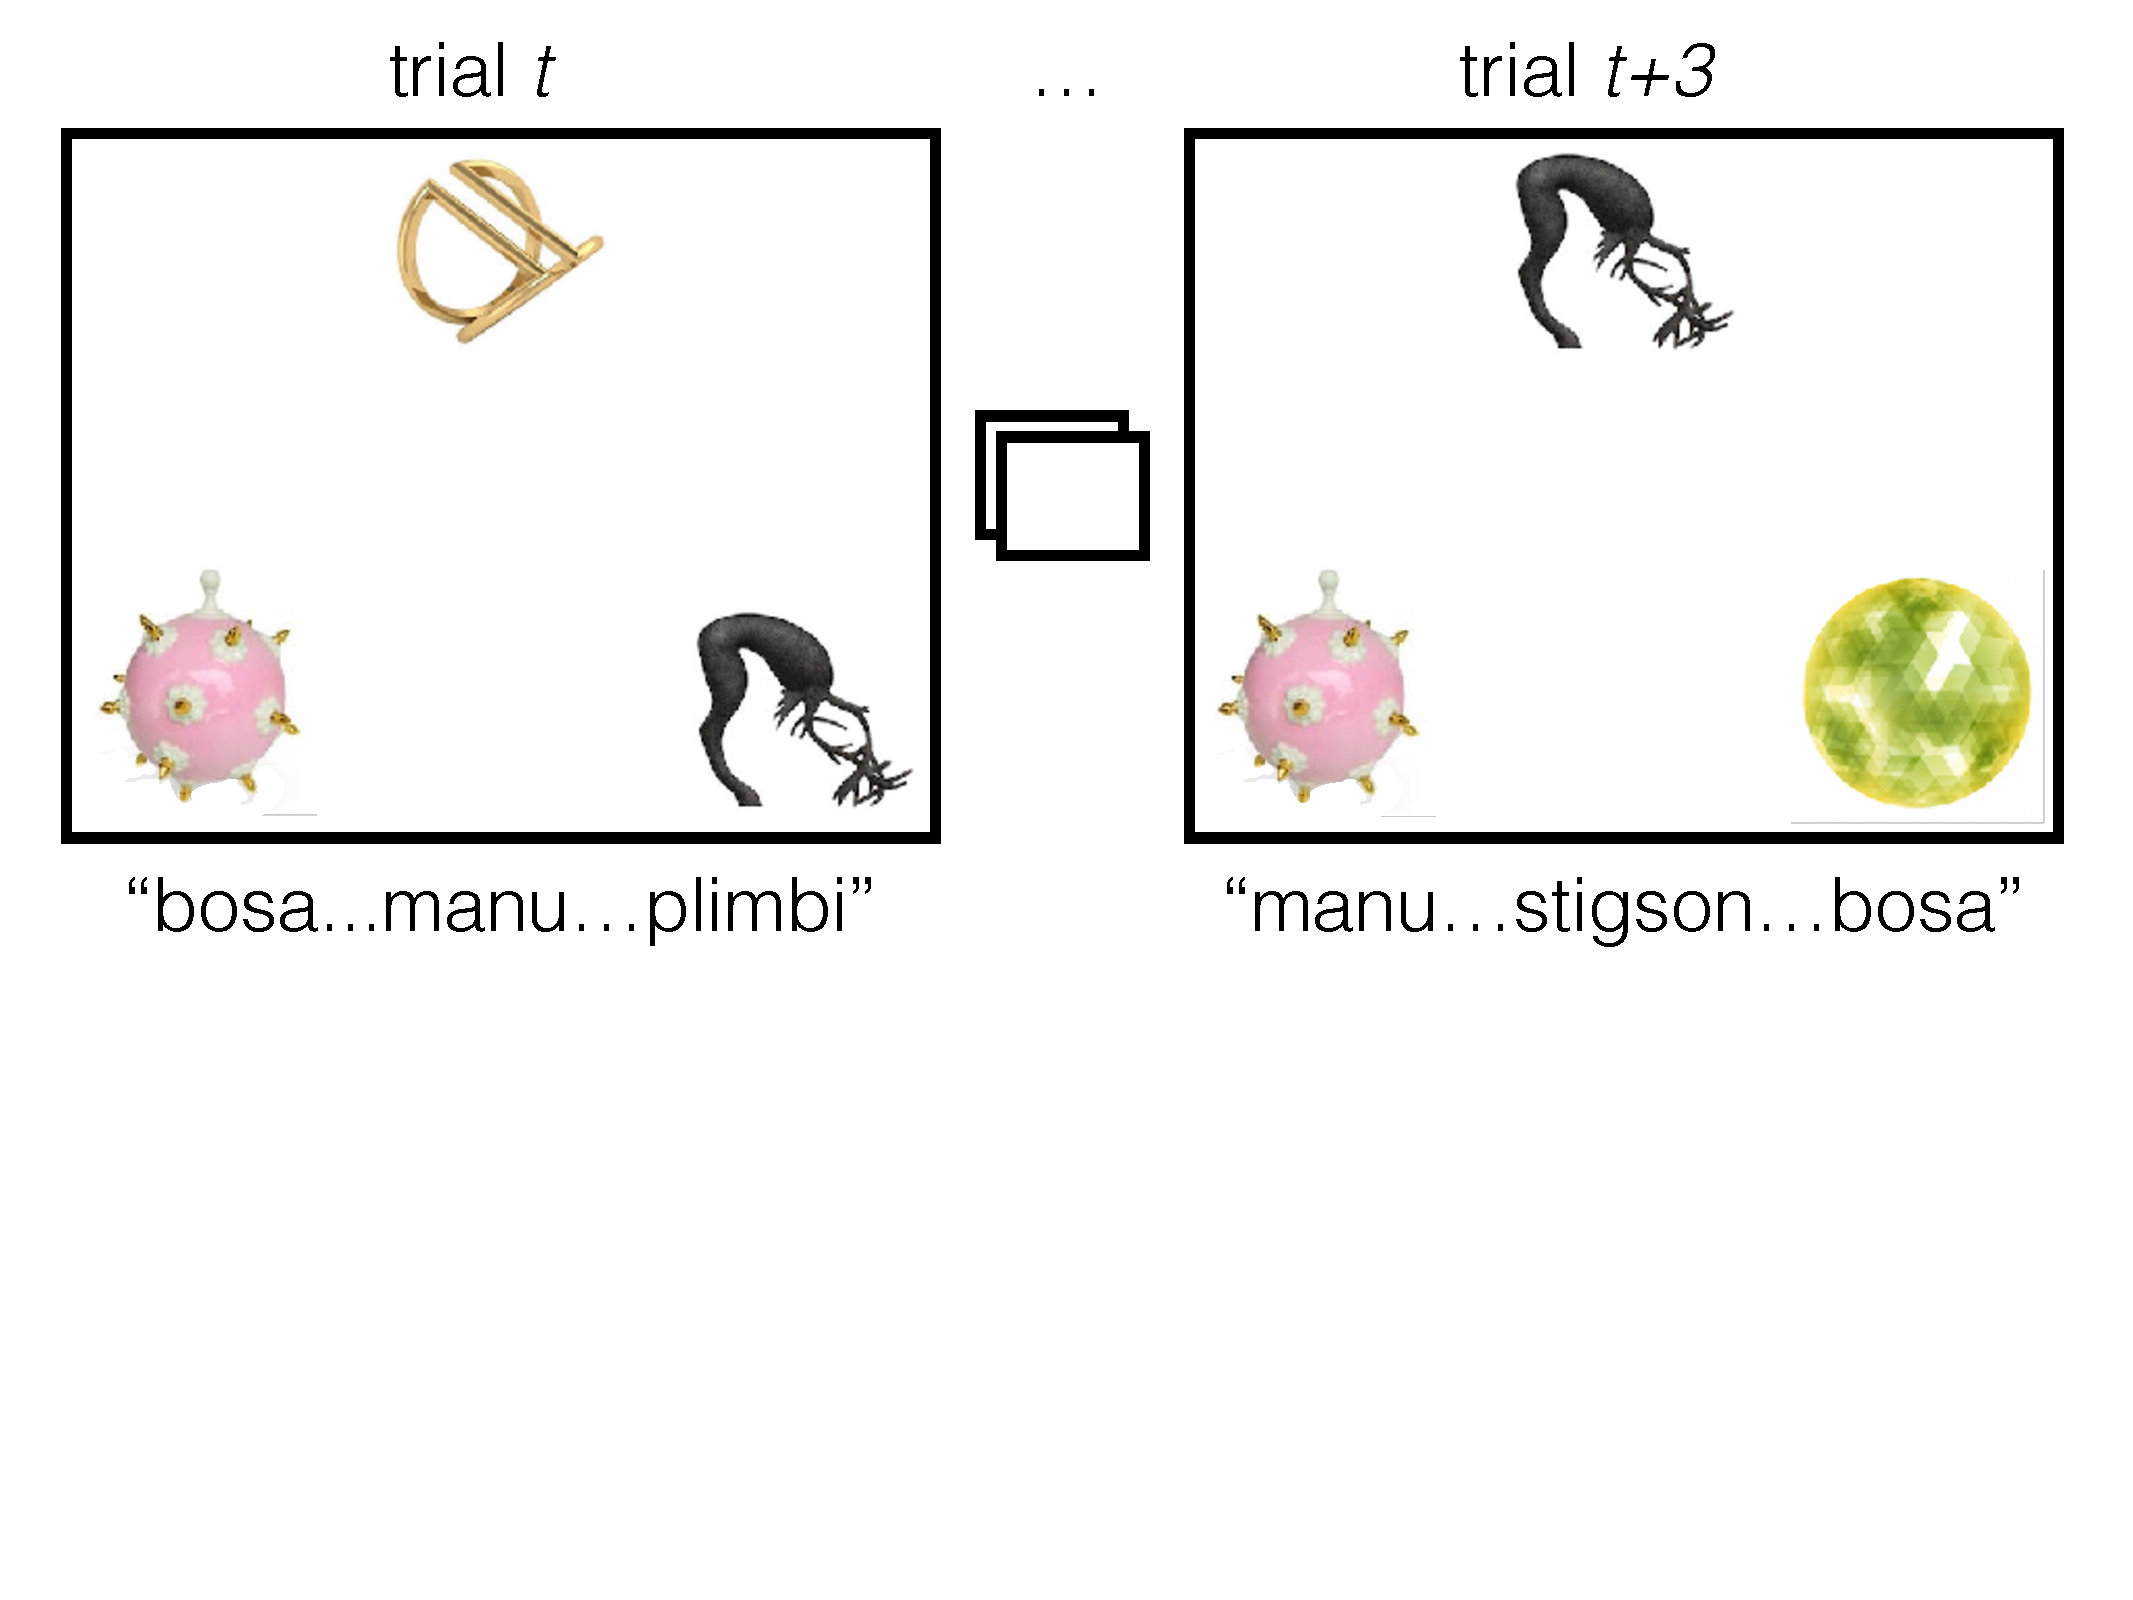
\includegraphics[width=0.65\textwidth]{intro_example}
  \caption{Example of two typical passive cross-situational training trials. On trial $t$, participants observe three objects and hear three pseudowords (``bosa, manu, plimbi''). Two intervening trials (not shown) each present three other objects and words, and then on trial $t+3$ two of the objects and words from trial $t$ are presented again alongside another object and word. Participants are tasked with learning which words refer to which objects, and cognitive models propose different accounts of how they accomplish this.}
  \label{fig:intro_example}
\end{figure} 

In the associative learning view, learners approximately store word-object associations between all co-occurring stimuli \citep{Yu:2008,Fazly:2010,Kachergis:2012vc,Kachergis:2012gi}. Such associative models assume that although every stimulus makes an impression, these associative memories compete with each other at test, causing retrieval failures. Moreover, some associative models apply attentional biases at learning so that not all co-occurrences are stored with equal strength. For example, \cite{Kachergis:2012gi} offers a model that has competing biases to attend to familiar word-object associations (i.e., strong from prior exposure), but also devotes storage more to stimuli with uncertain associates (e.g., novel stimuli). Importantly, this model assumes that learners are aware of their own state of (un)certainty about a word's associates. On the first example trial, this model would spread attention to all of the word-object associations equally, since all are novel and have no prior association. If prompted with $bosa$ after this trial, the model would select any of the three referents with equal probability--and is also aware of its own uncertainty via the entropy of the word's associations, which is used to drive future attention. On the second example trial, this model's familiarity bias would draw attention to strengthening all associations between ${manu, bosa}$ and ${o_2, o_3}$--all of which are familiar, but all of which will remain equally probable. However, the greater novelty of $stigson$ and $o_4$ also draw more attention to their conjunction ($stigson-o_4$), yielding an associative form of mutual exclusivity. Little attention is given to associations between the familiar and novel stimuli (e.g., $stigson-o_2$). This associative model shows a variety of trial order effects found in both word learning and associative learning studies, and thus may capture online learning \citep{Kachergis:2009tc,Kachergis:2012vc}.


Since the standard cross-situational learning task only measures knowledge in a final test at the end of training, it is difficult to infer the trial-by-trial learning dynamics. In the present study, we ask participants to indicate which object they believe each word refers to every time it occurs, allowing us to map out their developing knowledge over time. Of course, it is possible that this constant probing will affect task performance, but it is not a priori clear whether it will benefit or hinder learning. On the one hand, recognition memory research shows that being tested benefits memory more than a second study opportunity \citep{Carrier:1992}. On the other hand, asking learners to make a guess even on the first trial--when they cannot yet be certain of anything--may be tedious, or worse, misleading. Thus, we also compare learning in the continuous responding task to performance in the passive cross-situational learning task.

\section{Experiment}

In this experiment, we compare the standard cross-situational word learning paradigm, in which participants are {\em passively} trained by observing object displays co-occurring with words, to a {\em response} training condition in which participants are asked to choose one of the objects on display--or a ``Don't Know'' button--each time a word is heard during training. Although we use the same training statistics, it may be that performance on the two tasks will differ: it seems equally plausible that it is an advantage to be tested often, or that it may be a nuisance that distracts learners from remembering the co-occurrences. However, if performance on the two tasks is equal, it may be that the learning trajectories in the response condition can grant insight into the factors and mechanisms underlying cross-situational learning.

\subsection{Participants}

Participants in this experiment were 62 Indiana University undergraduate students who received course credit for their participation. None had participated in other cross-situational learning experiments.

\subsection{Stimuli and Procedure}

Verbal stimuli were 36 computer-generated pseudowords that are phonotactically-probable in English (e.g., ``bosa''), and were spoken by a monotone, synthetic female voice. Objects were 36 photos of uncommon, difficult-to-name objects (e.g., unusual tools or objets d'art). These 36 words and objects were randomly assigned to two sets of 18 word-object pairings; one set for each study condition. The entire set of stimuli from which the words and objects were randomly drawn is available online: \url{http://kachergis.com/downloads/stimuli.zip}.

Each training trial consisted of a display of four objects shown while four pseudowords were played in succession (see Figure~\ref{fig:trial}, though without the central ``Don't Know'' button), and 27 such trials were in each block. Although the words and objects in the two training conditions were different, their co-occurrence structure was the same: e.g., $w_1$ and $o_1$ appeared at the same trial indices and with the equivalent other stimulus pairs in both training conditions. In total, each of the 18 word-object pairs occurred 6 times during training. 

\begin{figure}[h]
  \centering
  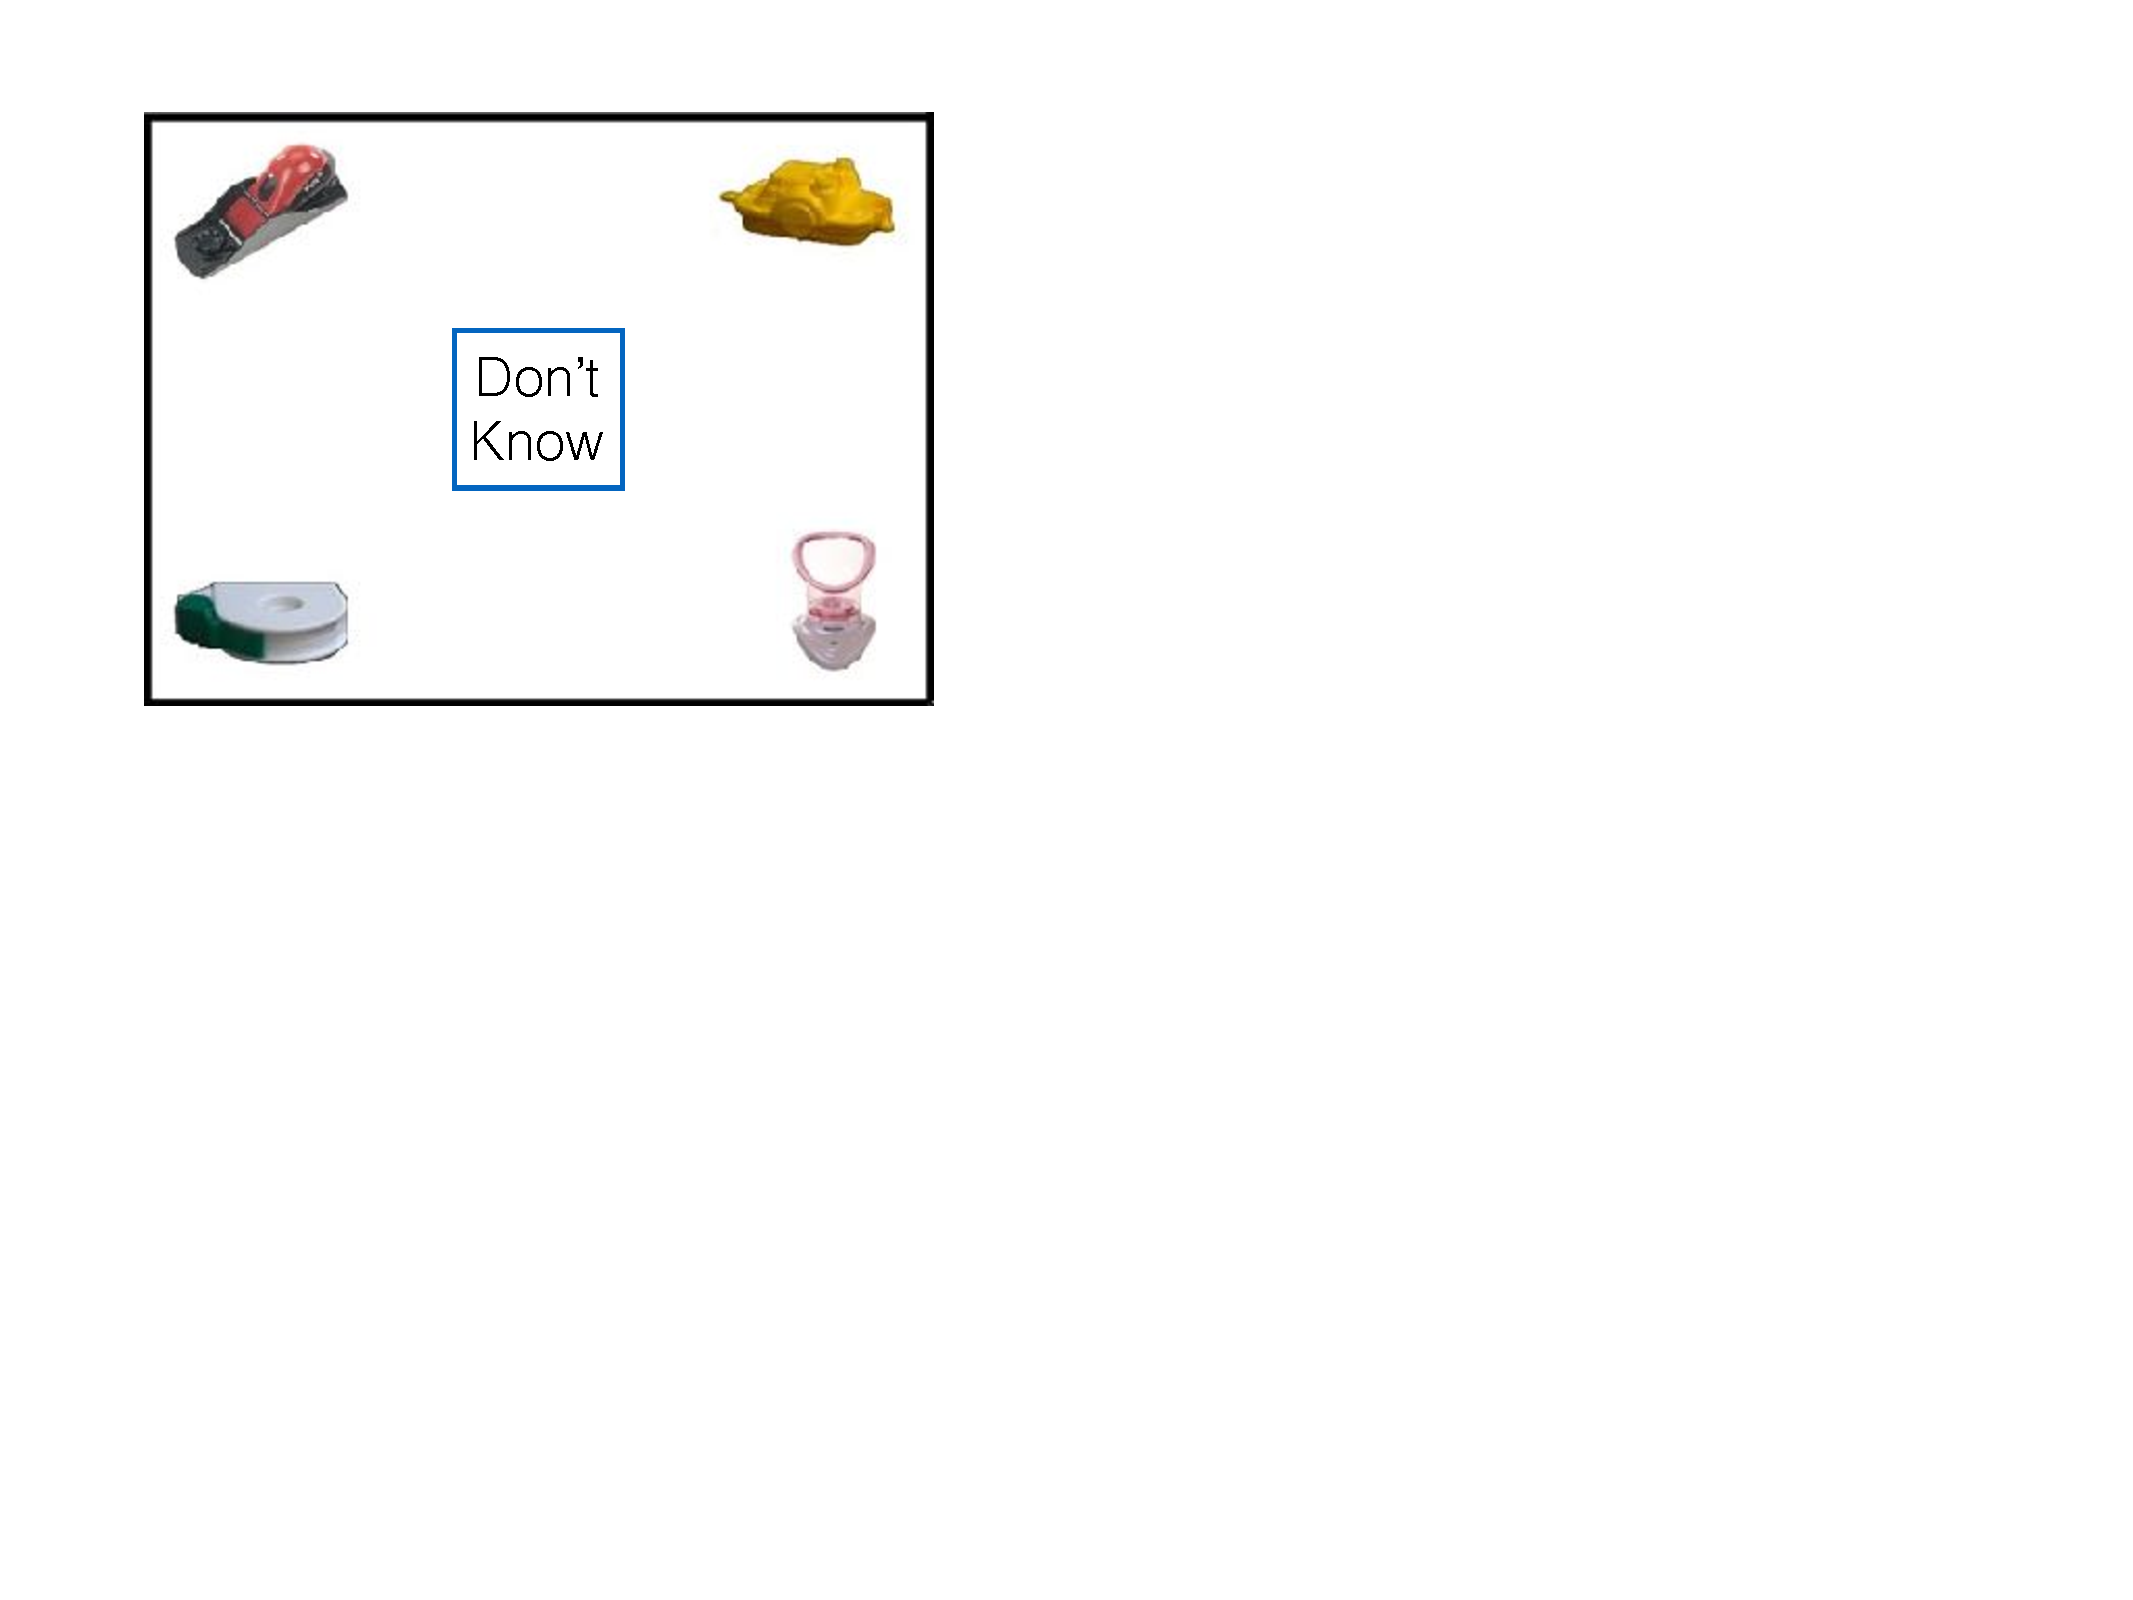
\includegraphics[width=0.35\textwidth]{task_diagram}
  \caption{Example training trial for the response condition, during which participants would hear four words (e.g., ``bosa..regli..manu..stigson''). The spoken words always referred to an object on the trial, but in a random order, making it impossible to disambiguate the assigned word-object mappings without cross-situational evidence. In the passive condition, no ``Don't Know'' button was visible, and participants were not instructed to respond after each word.}
  \label{fig:trial}
\end{figure} 

Training trials began with the appearance of four objects, which stayed onscreen the entire trial as words were heard (1 s duration, randomly ordered) after 2 seconds of initial silence. In the {\em passive training condition}, words were separated by 2 s of silence, for a total duration of 14 s per trial. Before training, participants were informed that they would see a series of trials with four objects and four alien words, and that their knowledge of which words refer to which objects would be tested at the end. 

Participants in the {\em response training condition} were additionally instructed that for each word during training, they were to choose with the mouse the best object, or click on the ``Don't Know'' button. In the response condition, after each word was heard the cursor appeared along with a ``Don't Know'' button in the center of the screen, as in Figure~\ref{fig:trial}, and participants were given unlimited time to click on one of the objects or the button. When a selection was made, the next word was presented.

After each training block, learners' knowledge was assessed using 18-alternative forced choice (18AFC) testing: on each test trial a single word was played, and the participant was instructed to choose from a display of all 18 objects the most appropriate one. A within-subjects design was used in order to see whether participants improved from one condition to the other. Condition order was counterbalanced.


\subsection{Results}

\subsubsection{Passive vs. Response Conditions}

Seven of the 62 participants were excluded for failing to perform above chance at the final test of either condition (18AFC chance performance $= .056$). Mean accuracy at the final test in the passive training condition for the remaining 55 participants was .31 (95\% Confidence Interval [.25, .37], which was not significantly different than mean accuracy in the response condition: .35 (95\% CI [.30, .41]; $t(54) = 1.03$, $p=.31$). Because these two conditions result in nearly equal performance and have the same statistical structure despite the major difference of responding throughout training, it may be that we can predict performance in one condition from performance in the other. As a first look at this, we examined the correlation between individual subjects' performance in the two conditions, but it was not significantly correlated ($r = .04$, $t(53)=.30$, $p=.77$). However, it turned out that there was a condition order effect: subjects showed worse performance in the first training condition, regardless of which condition it was (response mean: .27 vs. passive mean: .24), than in their latter training condition (response: .40 vs. passive: .43). This general improvement from one condition to the next makes it unsurprising that there is little correlation between subjects' performance in the two conditions. It also suggests that the tasks are similar enough that practice on the earlier helps the latter--whatever the order. There was also no significant correlation between the performance on statistically-equivalent test items (word-object pairs) in the two conditions ($r = -.21$, $t(16)=-.84$, $p=.41$). The maximum accuracy for an item (.51) was in the response condition, and the minimum (.24) was achieved by a unique item in each condition. This lack of consistency between the passive and response conditions could result from different strategies/mechanisms being used in each condition, or simply because the random learning trajectory taken by each learner varies too much.

The remainder of our analyses focus on the response condition data, which allow us to investigate several additional interesting questions, such as: Of the pairs that were known on the final test, how many repetitions were required for learning? Was there evidence that some well-learned pairs were forgotten at the final test? How many pairs were typically learned on a given training trial--in general, and over time? 


\subsubsection{Training Responses}

The median time to make a response after word onset on a training trial was 1869 ms (mean: 2416 ms), similar in duration to the 2000 ms between words on a training trial in the passive condition. 42\% of the responses during training were incorrect, 38\% were correct, and 20\% were ``Don't Know'' responses. On average, learners' median response times were fastest on correct responses (1745 ms), faster than incorrect responses (2117 ms; paired $t(54)=5.49$, $p<.001$), which were faster than ``Don't Know'' responses (2830 ms; paired $t(54)=2.84$, $p<.01$). The fact that the uncertain responses are slowest may indicate that participants use this option when they realize that none of the presented objects are strongly associated with the given word, or in the hypothesis-testing view, that learners failed to retrieve a hypothesized meaning for that word.

The first time each word was heard, participants were more likely to use the ``Don't Know'' button (proportion on first occurrence: .37 vs. all later occurrences: .17, $t(54) = 5.83$, $p<.001$), showing some awareness that they had no basis on which to hypothesize a meaning for that word. The first four training trials contained 16 unique items. Only when the remaining two items first appeared could learners could in principle use novelty-based inference to make a principled hypothesis. The mean proportion of correct and incorrect responses on the first occurrence was .20 and .44, respectively--showing that many participants are willing to guess, even when they cannot yet know the correct meaning. On the second occurrence of each word, we investigated the conditional probability of correct, incorrect, and uncertain responses as a function of their response on the first occurrence of the word. Table~\ref{tab:condprob} shows the probability of each response on the second occurrence of each pair, conditioned on the first response.  We had two hypotheses in mind: 1) that they would be more likely to be correct on the second response if they were previously correct, and 2) that even for incorrect or uncertain responses, they may be more likely to select the correct referent--since they have acquired some knowledge. 

\begin{table}[ht] 
\begin{center}
\caption{Conditional probability of response on the second training occurrence given the response on the first occurrence.} 
\label{tab:condprob} 
\vskip 0.05in
\begin{tabular}{c | c c c | c | c}
&  \multicolumn{3}{|c|}{Probability of Second Response} & & \\
 \hline
First Response   &  Correct & Uncertain & Incorrect & N & Final Accuracy \\
\hline 
Correct	 &   0.50  &   0.09   &   0.41 &  182    &     0.49     \\
Uncertain  &   0.20  &   0.41   &    0.39 &  337    &     0.36     \\
Incorrect 	 &   0.29  &   0.11   &    0.60 &  411    &      0.28    \\
\hline
\end{tabular} 
\end{center}
\end{table}

Learners who were correct on the first occurrence were correct on the second occurrence for 50\% of the items, greater than the 20\% that were correct on the second after being uncertain on the first (Welch's $t(78.3)=5.30$, $p<.001$) or than the 29\% that were correct after being incorrect on the first (Welch's $t(85.05=3.29$, $p=.001$). This matches a result in a somewhat differently-structured paradigm in \cite{Trueswell:2013}, which found that learners were at chance when selecting a referent for a word they had been wrong about on the previous occurrence. Among other differences (e.g., familiar objects were used), that paradigm did not allow learners to choose a ``Don't Know'' option. Nonetheless, it is good to replicate this result in our response paradigm.


To see if this pattern of results holds for successive responses, in general, we calculated the probability of each response type (on occurrence 2 through 6) given the previous response type (on occurrence 1-5). Shown in Table~\ref{tab:condprob_all}, these conditional probabilities are quite similar to those calculated for the first and second responses alone: learners who were correct on the previous response were quite likely to respond correctly on the current response (0.66, compared to 0.27 after an incorrect response). Analogously, responding incorrectly was most likely to yield an incorrect next response (0.58), with a 30\% chance of transitioning to a correct response. Now that we have examined the overall transition probabilities in responding during training, we compare learning trajectories for pairs that were known at the final 18AFC test to those that were not finally known.

\begin{table}[ht] 
\begin{center}
\caption{Probability of response on the current training occurrence (2-6) given the response on the previous occurrence (1-5).} 
\label{tab:condprob_all} 
\vskip 0.05in
\begin{tabular}{c | c c c | c }
&  \multicolumn{3}{|c|}{Probability of Current Response} & \\
 \hline
Prev. Response & Correct & Uncertain & Incorrect  & N \\
\hline 
Correct	 & 0.66 & 0.07  &   0.27  & 1,694    \\
Uncertain  & 0.23 & 0.41  &   0.36   & 1,063    \\
Incorrect 	 & 0.30 & 0.12  &   0.58  & 2,133    \\
\hline
N              &   808 &   2,065 & 2,017  \\ 
\hline
\end{tabular} 
\end{center}
\end{table}


\subsubsection{Learned vs. Not Learned Pairs}

In the response condition, what patterns of responses during training separate pairs that were known at the final 18AFC test from those that were not known? We measured a few statistics for each pair, and measured their correlation with accuracy for that pair on the final test across all subjects. The statistics we included for each pair are: the occurrence when its object was first correctly chosen (1-6, 7 if never; First Learned), how many times the correct object was selected for that word (0-6; Correct), the number of times an incorrect object was selected for that word (0-6; Incorrect), and the number of times ``Don't Know" was selected for the word (0-6; Don't Know). These item-level statistics concerning responses during training were averaged for each subject and correlated with accuracy on the final 18AFC test for those items in the response condition. Figure~\ref{fig:test_acc} shows that mean accuracy on the final 18AFC test increased the more often a word's referent was correctly selected during training (Correct; $r=.66$, $t(310)=15.37$, $p<.001$), and that all other measures were negatively correlated. Selecting the incorrect object more often resulted in lower accuracy on the final test ($r=-.58$, $t(290)=12.13$, $p<.001$). Similarly, choosing the ``Don't Know'' button more often was correlated with lower test accuracy ($r=-.29$, $t(203)=4.33$, $p<.001$). Correctly selecting the object earlier (First Learned; occurrence 1-6, or 7 if never) resulted in higher test accuracy ($r=-.35$, $t(324)=6.77$, $p<.001$).

\begin{figure}[h]
  \centering
  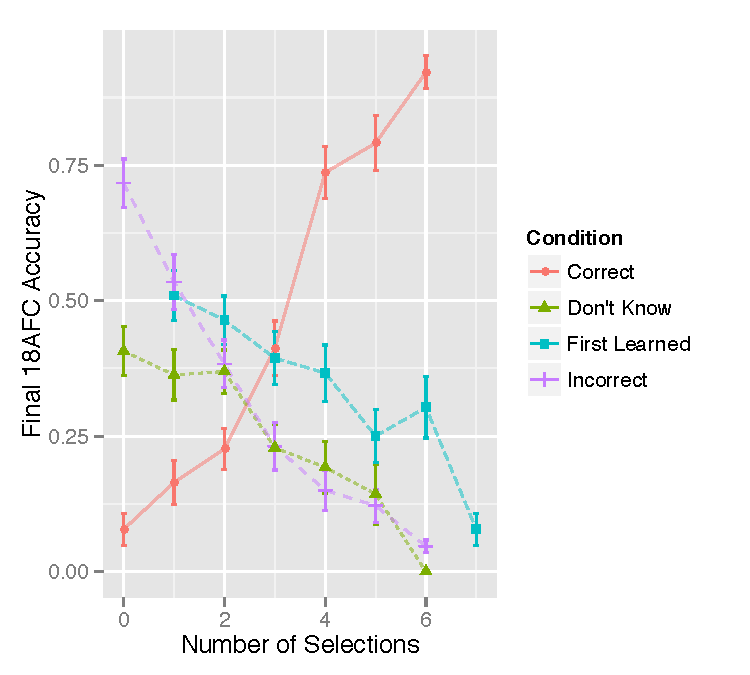
\includegraphics[width=0.6\textwidth]{responses_vs_final_acc}
  \caption{Accuracy on final 18AFC test as a function of different statistics about that item's responses during training. Correctly selecting the referent more than three times in training resulted in $\geq75\%$ accuracy on final test.}
  \label{fig:test_acc}
\end{figure} 

\subsubsection{Clustering Item Response Profiles}

Given that these aggregate statistics of online responding are predictive of final 18AFC accuracy, we chose to look for types of response profiles by clustering the individual items according to these item-level statistics (i.e., first learned, correct selections, incorrect selections, and ``Don't Know'' selections), and then investigating the discovered clusters to see if their final accuracy differed. Partitioning around medoids \citep{fpc} found four response profiles, with the number of clusters being estimated by the optimum average silhouette width method \citep{silhouette}. Shown in Table~\ref{tab:clusters}, items in three of the clusters (2-4) have fairly low final 18AFC performance (cluster 2: 0.25, cluster 3: 0.19 and cluster 4: 0.14). In terms of their online response characteristics, these low-performing item clusters have a low number of average correct responses (2.03, 0.78, and 0.40, respectively) and a late average First Learned occurrence (2.71, 5.75, and 6.51). The average item in cluster 4 was not even correctly chosen once during training (because the mean is greater than 6.51), whereas cluster 2 actually had a mean first-learned index of 2.71--and a higher final accuracy (0.25 compared to cluster 4's 0.14). In contrast, cluster 1's 252 items--with 78\% final 18AFC accuracy--were first-learned by occurrence 1 or 2 (mean: 1.71), and were correctly responded to a mean of 4.73 times during training. In summary, although the item clusters do not perfectly predict final 18AFC accuracy, the three clusters with below-chance performance (clusters 2, 3, and 4) generally contained items with late-learned, and either oft-incorrect or oft-uncertain responses, whereas the cluster with high final performance (cluster 1) mostly consisted of early-learned, never-forgotten pairs. 

\begin{table}[ht] 
\begin{center}
\caption{Training statistics of clustered items.} 
\label{tab:clusters} 
\vskip 0.05in
\begin{tabular}{c c c c c c c}
\hline
                & First  & Correct               & Incorrect  & ``Don't  & Finally  &  \\
 Cluster  & Learned &  Responses &  Responses & Know'' &  Correct & N \\
\hline
       1  &   1.71    &    4.73 &  0.69     &       0.48    &      0.78  & 252 \\
       2  &    2.71   &    2.03 &  3.16     &       0.77    &      0.25  & 418 \\
       3  &   5.75    &    0.78 &  1.25     &       3.88    &      0.19  & 153 \\
       4  &   6.51    &    0.40 &  4.78     &       0.80    &      0.14  & 167 \\
\hline
\end{tabular} 
\end{center}
\end{table}



Motivated by the existence of high- and low-performing clusters, as selected solely by their response patterns during learning, we chose to examine and model mean response trajectories, occurrence-by-occurrence, split by finally-learned and finally-unknown items. Shown in Table~\ref{tab:train_acc}, and in Figure~\ref{fig:train_by_final_acc}, these response trajectories show stark differences for finally-correct vs. finally-incorrect items. Finally-correct items (35\% of the items) start at chance correctness on the first training occurrence, and then exhibit steadily-increasing correct responding across training. In contrast, the finally-incorrect items have incorrect responses half the time across training, consistently from the first through the last occurrence. Nonetheless, some of the finally-incorrect items show increasing correct responses over training.

By testing theoretically-derived computational models of learning, we can determine which underlying mechanisms are capable of explaining human behavior in this task. Namely, the key features of the behavioral data are: 1) learning looks incremental, and 2) responses during training reflect what learners know moment by moment -- including what they know they don't know. In the next section, we fit two models---representing the hypothesis and associative views of word learning---to the mean training response proportions (correct, incorrect, and uncertain for both finally-correct and finally-incorrect items; shown in Table~\ref{tab:train_acc}) and final 18AFC accuracy (0.345), to see which mechanisms better account for the results.


\begin{figure}[h]
  \centering
  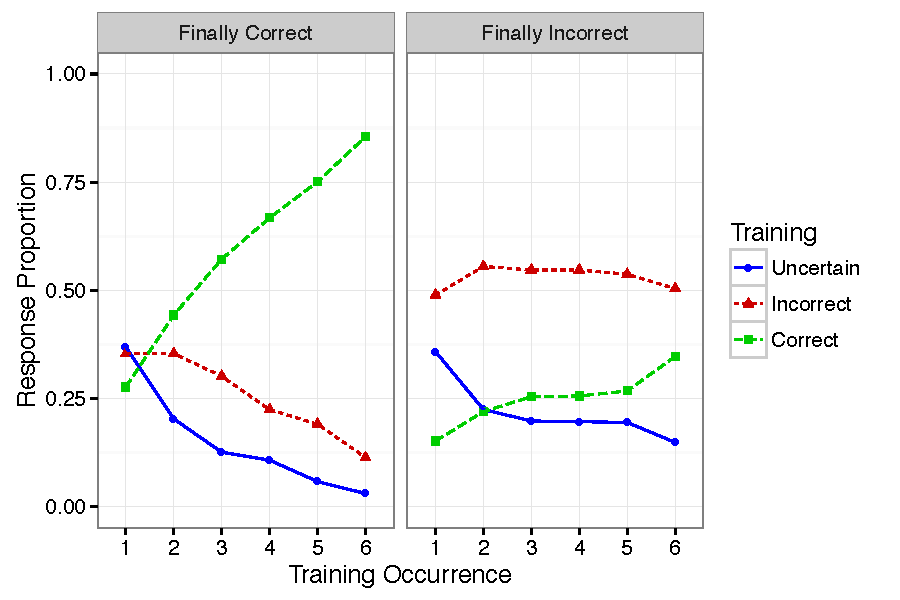
\includegraphics[width=0.7\textwidth]{human_training_responses_by_final_acc}
  \caption{Response utilization during training for items that were known or unknown on the final 18AFC test. The 35\% of items that were finally correct showed increasingly correct responses during training, whereas the 65\% of items that were finally incorrect showed constant, high levels of incorrect responding during training.}
  \label{fig:train_by_final_acc}
\end{figure} 


\begin{table}[ht] 
\begin{center}
\caption{Training response by occurrence and accuracy on final test.} 
\label{tab:train_acc} 
\vskip 0.05in
\begin{tabular}{l | c | c  c c c c c}
\hline
{\em Final} & Training & \multicolumn{6}{c}{Occurrence} \\
{\em Test} & Resp. &   1   &  2  &  3  &  4  &  5  &  6 \\
\hline
\multirow{2}{*}{{\em Correct}} & Correct & .28 & .44 & .57 & .67 & .75 & .86 \\
				 	  & Uncertain & .37 & .20 & .13 & .11 & .06 & .03 \\
				(.35)	   & Incorrect  & .35 & .36 & .30 & .22 & .19 & .11 \\
\hline
\multirow{2}{*}{{\em Incorrect}} & Correct & .15 & .22 & .25 & .26 & .27 & .35 \\
				     	& Uncertain & .36 & .22 & .20 & .20 & .20 & .15 \\
				(.65)     & Incorrect  & .49 & .56 & .55 & .54 & .53 & .5 \\
\hline
\end{tabular} 
\end{center}
\end{table}


\section{Models}

We compare recent models representing competing intuitions about word learning. As discussed in the introduction, the hypothesis-testing view holds that learners only store a single hypothesized meaning for each word \citep{Medina:2011,Trueswell:2013}. Hypotheses are chosen from available objects on a trial, but only if that referent is not already linked to another word. In the purely associative view, multiple possible meanings for a word accumulate in memory, on each trial \cite[e.g.,][]{Smith:2000,Yu:2008}: each word can become associated with all of the presented objects, although perhaps not equally \citep{Kachergis:2012gi}.  At test, a given word's associations with multiple objects compete, making recall probabilistic. After describing two hypothesis-testing models and two versions of the biased associative model, we test how well each model is able to fit the proportion of correct, uncertain, and incorrect responses humans made at each occurrence of a word, split by finally-correct and finally-incorrect items (as shown in Table~\ref{tab:train_acc} and in Figure~\ref{fig:train_by_final_acc}), as well as the proportion correct for each pair on the final 18AFC test (mean = 0.345).



\subsection{Hypothesis Testing Models}

\cite{Medina:2011} laid out the assumptions of a class of hypothesis testing models:

\begin{quote}
``(i) learners hypothesize a single meaning based on their first encounter with a word; (ii) learners neither weight nor even store back-up alternative meanings; and (iii) on later encounters, learners attempt to retrieve this hypothesis from memory and test it against a new context, updating it only if it is disconfirmed. Thus, they do not accrue a ``best" final hypothesis by comparing multiple episodic memories of prior contexts or multiple semantic hypotheses." (p. 3)
\end{quote}

\subsubsection{Guess-and-Test Model}

We test a {\em guess-and-test model} based on the above assumptions stated by \cite{Medina:2011} that we previously implemented in \cite{Kachergis:2012hyp}.
This model is also quite similar to the model tested in simulations of learning a full-sized vocabulary by \cite{Blythe:2010il}, with differences noted below. In the guess-and-test model, when word $w$ is heard during training the guess-and-test model retrieves the stored hypothesis $w-o_h$ with probability $1-f$. With probability $f$, $w-o_h$ fails to be retrieved and is forgotten. If $w-o_h$ is retrieved but $o_h$ is not on the trial, the hypothesis is erased. After a given trial's retrieval attempts are completed, objects on that trial that are not part of an existing hypothesis are randomly assigned without replacement to any words now without a hypothesis, effecting a local mutual exclusivity constraint. Each new hypothesis is successfully stored with probability $s$. Thus, the free parameters in the model govern probabilistic storage ($s$) and forgetting ($f$) of hypotheses.\footnote{\cite{Blythe:2010il} assumed for ease of analysis that learners do not suffer failures at storage or retrieval.} 
The final 18AFC test is straightforward: the model simply chooses the hypothesized object for each word, and chooses randomly from objects that have no name if there is no hypothesis stored for the current word. Responses during training are handled similarly (i.e., the currently-stored hypothesis for each word is chosen, resulting in correct and incorrect responses), except that an uncertain response is made with probability proportional to an additional parameter, $\gamma$, that we add in order to model learners' usage of the ``Don't Know'' button. Since the stored hypotheses gain weight if they are verified, the fixed value of $\gamma$ can result in a dropping rate of uncertain responding. Few other mechanisms for making uncertain responses in the propose-but-verify model can be implemented, since each word has only one hypothesis stored at a given time.

\subsubsection{Propose-but-Verify Model}

More recently, \cite{Trueswell:2013} introduced the {\em propose-but-verify model}, another formalism of the same hypothesis-testing assumptions. The propose-but-verify model of cross-situational learning begins by guessing and storing a single hypothesized object for each word on a trial. When a word appears again, the previous guess is recalled with some probability $\alpha_0$. If the recalled hypothesis is present on the trial, $\alpha_0$ is increased by an amount $\alpha_r$. If the object fails to be recalled, or is recalled but not present, a new referent is selected--but only from objects that are not currently linked to a word.

The propose-but-verify model assumes that learners store a list of word-object pairs, with only up to one object stored for a given word. At the beginning of training, this list is empty. On each training trial, for each presented word $w$ the learner retrieves the hypothesized object $o_h$ with probability $\alpha_0$ (or $\alpha_0 + \alpha_r$, if $w-o_h$ has been previously retrieved). If $o_h$ fails to be retrieved, the hypothesis $w$-$o_h$ is forgotten. If $o_h$ is retrieved, but is not present on the trial, the hypothesis $w$-$o_h$ is erased. For any words on a trial now without a hypothesis ($w_N$), new hypothesized objects are chosen\footnote{Randomly without replacement--a local mutual exclusivity constraint.} from those objects that are not part of a hypothesized pairing. Thus, the model can bootstrap: if three of four objects on a trial are successfully retrieved, the final object will be assigned to the word that has no hypothesized meaning. 
An additional parameter ($\gamma$) was used to threshold uncertain responses, exactly as in the guess-and-test model. 


\subsection{Associative Models}

An unbiased associative model might simply strengthen associations between all presented words-object pairings on a trial by a constant amount, essentially tracking co-occurrences in a word $\times$ object associative memory matrix. Here we instead consider the biased associative model introduced by \cite{Kachergis:2012gi}, which assumes that learners do not attend equally to all presented word-object pairings. Thus, although all co-occurrences are registered to some extent in memory, greater attention and storage is directed to pairings that have previously co-occurred. Moreover, this bias for familiar pairings competes with a bias to attend to stimuli that have no strong associates (e.g., novel stimuli). Familiar associations demand more attention than pairings that have not been associated before. However, attention is also pulled individually to novel stimuli because of the high uncertainty of their associations (i.e., they have diffuse associations with several stimuli). The level of uncertainty is quantified by the entropy of a stimulus' association strengths, and attention is allocated to objects and words in proportion to these entropies.

Formally, given \textit{n} words and \textit{n} objects to be learned over a series of trials, let \textit{M} be an \textit{n} word $\times$ \textit{n} object association matrix in which associations accumulate during training. Cell $M_{w,o}$ will be the strength of association between word \textit{w} and object \textit{o}. Strengths are augmented by viewing the particular stimuli. \textit{M} is initialized with zeros. On each training trial \textit{t}, a subset \textit{S} of \textit{m} word-object pairings appears. If there are any new words and objects are seen, new rows and columns are first added. The initial values for these new rows and columns are \textit{k}, a small constant (here, 0.01). 

Association strengths are allowed to decay, and on each new trial a fixed amount of associative weight, $\chi$, is distributed among the associations between words and objects, and added to the strengths. The rule used to distribute $\chi$ (i.e., attention) balances a preference for attending to `unknown' stimuli with a preference for strengthening already-strong associations. When a word and referent are repeated, extra attention (i.e., $\chi$) is given to this pair---a bias for prior knowledge. Pairs of stimuli with no or weak associates also attract attention, whereas pairings between less-known objects and more-known words, or vice-versa, do not attract much attention. To capture how well-known a stimulus is, strength is allocated using entropy (\textit{H}), a measure of uncertainty that is 0 when the outcome of a variable is certain (e.g., a word appears with one object, and has never appeared with any other object), and maximal ($log_2 n$) when all of the $n$ possible object (or word) associations are equally likely (e.g., when a stimulus has not been observed before, or if a stimulus were to appear with every other stimulus equally). In the model, on each trial the entropy of each word (and object) is calculated from the normalized row (column) vector of associations for that word (object), \textit{p}(\textit{M$_w,\cdot$}), as follows:

\begin{equation}
  H(w) = - \sum_{i=1}^{n} p(M_{w,i}) \cdot \textnormal{log}( p(M_{w,i} ) )
  \label{eqn:entropy}
\end{equation}

As in \cite{Kachergis:2012gi}, the trial-to-trial update rule for adjusting and allocating strengths for a presented word-object ($w,o$) pair is:

\begin{equation}
  M_{w,o,t+1} =  \alpha M_{w,o,t} + \frac{ \chi \cdot e^{ \lambda \cdot (H(w) + H(o)) } \cdot M_{w,o,t}  }{  \sum_{w\in W} \sum_{o\in O} e^{ \lambda \cdot (H(w) + H(o)) } \cdot M_{w,o,t} }
  \label{eq:fullmodel}
\end{equation}

In Equation~\ref{eq:fullmodel}, $\alpha$ is a parameter governing forgetting, $\chi$ is the weight being distributed, and $\lambda$ is a scaling parameter governing differential weighting of uncertainty ($H(\cdot)$; roughly novelty) and prior knowledge ($M_{w,o,t}$; familiarity at trial $t$). As $\lambda$ increases, the weight of uncertainty (i.e., the exponentiated entropy term, which includes both the word and object's association entropies) increases relative to familiarity. The denominator normalizes the numerator so that exactly $\chi$ associative weight is distributed among the potential associations on the trial. For stimuli not on a trial, only forgetting operates. After training and prior to test, a small amount of noise (\textit{c = }.01 here) is added to \textit{M.} At test, learners choose one referent for each word from the \textit{m} alternatives, in proportion to their associative strengths to the word. 

To make responses during training, after updating associations on the trial according to Equation~\ref{eq:fullmodel}, the model chooses an object for each word with probability proportional to the strength of the word's association with that object, or chooses the uncertain response with probability proportional to the word's uncertainty (Shannon entropy, as defined above, but only for the objects on the trial), scaled by parameter $\gamma$. The $\gamma$ parameter is thus only used to make ``Don't Know'' responses during training, scaling the relative influence of stimuli's association entropies relative to the association strengths--not playing any role in learning. This is analogous to the mechanism we employ in the propose-but-verify model for making uncertain responses during training, except that the underlying representation of the associative model is richer: to guide learning, the model has multiple graded associations and an awareness of its uncertainty across these associations.

It should be noted that the associative model above describes trial-level learning, capturing the relative attention given to particular word-object pairings on a trial. At a more detailed level, as they hear words learners are no doubt making eye movements to particular objects, sampling from the available word-object pairings (perhaps according to the familiarity of the pairing and the stimulus uncertainty). Because the data we are considering is now closer to this level of granularity, we chose to test two versions of the associative model. Exactly as defined above, the {\em associate all referents} updates associations between each presented word and all appearing objects. 
In the {\em associate one referent} model, a single association for each presented word per trial is sampled (with replacement, and with probability proportional to the association strength) from the memory matrix. Thus, both models use the same update strength- and uncertainty-biased update rule, but now the {\em associate one referent} version of the model is only updating a single association per word, per trial.

\section{Model Results}

Using a differential evolution search algorithm \citep{deoptim} we sought optimal\footnote{Note that although differential evolution  optimization is not guaranteed to converge on optimal values, in our experience it has found better and more stable estimates than other search algorithms, many of which require assumptions about the problem being optimized (e.g., differentiability) that cognitive models rarely meet.} parameter values for both models in order to minimize the discrepancy between the models' and humans' proportion of correct, incorrect, and uncertain responses across training, shown in Table~\ref{tab:train_acc}, along with the final proportion correct for each of the 18 word-object pairs at test (mean = 0.345).
The disparity between model-predicted and observed response proportions was measured using log-likelihood. BIC, a criterion for model selection based on fit with a penalty for the number of free parameters, was used to select the best model.

The best-fitting parameter values found for all four models are shown in Table~\ref{tab:model_fits}, along with BIC values and the models' predicted final test (18AFC) accuracy.
The propose-but-verify model had the worst BIC = 87.01, and a final 18AFC accuracy of 0.41. The best-fitting parameter values found for the guess-and-test model were $s = .17$ and $f = .37$--a quite low storage probability and moderate rate of forgetting--and $\gamma = .37$, with BIC = 86.29, and final 18AFC accuracy of .36. Shown in Figure~\ref{fig:human_vs_models}, the guest-and-test model's response trajectories are similar to humans', but with two notable exceptions: 1) correct responding to finally-correct items reaches ceiling in the model, and 2) correct responding to finally-incorrect items stays flat (or even decreases), whereas humans show gradual increase. Accuracy on final 18AFC test of the guess-and-test model does closely match humans (0.36 to people's 0.345), while the propose-but-verify model's final accuracy was higher (0.41).
BIC strongly prefers the biased associative model that updates a single referent per word (BIC = 79.16) over either hypothesis-testing model, despite its additional parameter. The associative model that updates all referents per word is also preferred (BIC = 82.30) over the hypothesis-testing models, but fits less well than the one-referent associative model, predicting little difference between finally-correct and finally-incorrect items, whereas humans show much slower learning for finally-incorrect items.
As seen in Figure~\ref{fig:human_vs_models}, all but the associate-all-referents model match the response trajectories for finally-correct items fairly well, although note that for finally-incorrect items (right panels), the propose-but-verify model (top right) shows a marked drop--to 0--in correct responses at the final training occurrence, which is not present in the human data. Like humans, the associate-one-referent model's finally-incorrect items show slow but increasing correct responding, including at the final training occurrence. 

\begin{table}[ht] 
\begin{center}
\caption{Best-fitting parameter values, performance, and BIC for each model.} 
\label{tab:model_fits} 
\vskip 0.05in
\begin{tabular}{c | c | c | c }
 \hline
Model & Best-fitting Parameter Values & 18AFC Accuracy & BIC  \\
\hline 
Guess-and-Test      & $s = .17$, $f = .37$, $\gamma = .37$ 				  		    & 0.36  &  86.29  \\
Propose-but-Verify  & $\alpha$ = 0.15, $\alpha_{incr}$ = 0.68, $\gamma$ = 0.05 		    & 0.41  &  87.01  \\
Assoc. One Referent & $\chi$ = 0.12, $\lambda$ = 0.18, $\alpha$ = 0.94,  $\gamma$ = 0.15 & 0.37 & 79.16   \\
Assoc. All Referents  & $\chi$ = 0.13, $\lambda$ = 21.18, $\alpha$ = 1.00, $\gamma$ = 0.11 & 0.33 & 82.30  \\
\hline
%Human              &  --  &  0.34  &  -- & -- \\ 
%\hline
\end{tabular} 
\end{center}
\end{table}


In summary, the associative model achieves a better quantitative and qualitative fit to the data than the propose-but-verify model offered by \citep{Trueswell:2013}, or by the earlier guess-and-test account based on the assumptions of \citep{Medina:2011}. In conclusion, we note that even slightly different formal models--propose-but-verify and guess-and-test stem from the same intuitions, and quite similar verbal descriptions--can result in quite different learning trajectories during training, helping us distinguish models. Thus, in addition to fitting final accuracy with a low chance baseline (e.g., 18AFC, as in the present study), it is useful to leverage trial-to-trial responses during training to additionally constrain model selection. 



\begin{figure}[h]
  \centering
  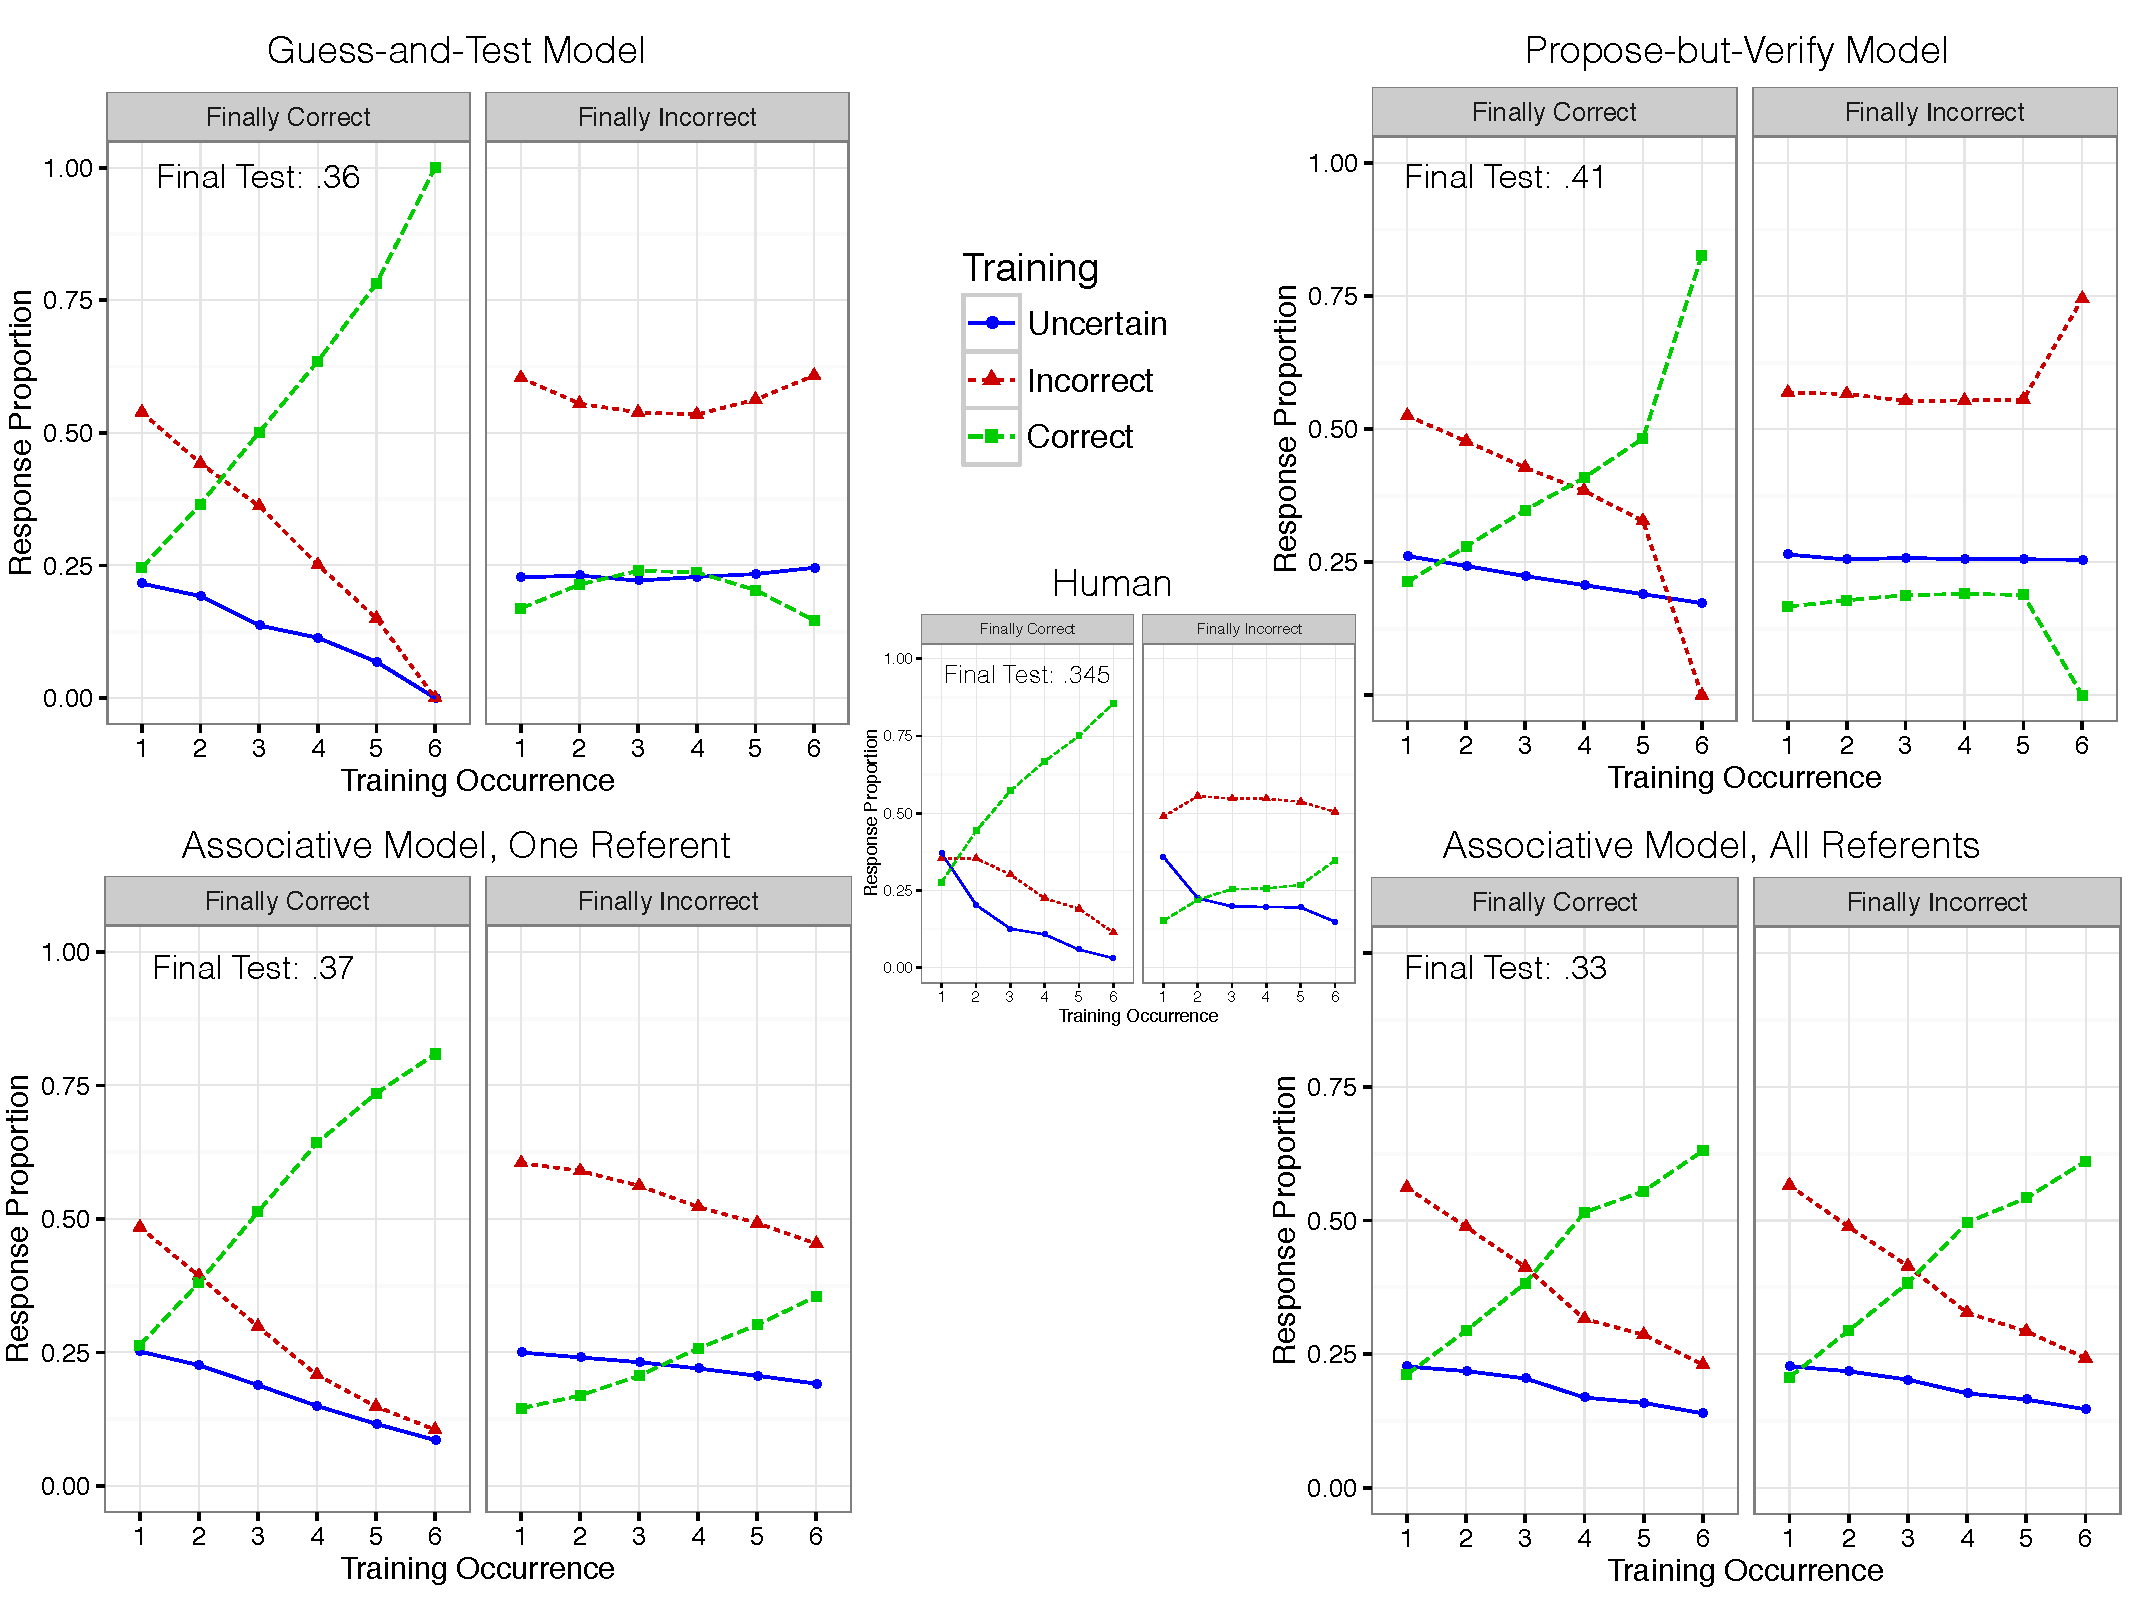
\includegraphics[width=0.95\textwidth]{response_graph_loglik_w_human}
  \caption{Hypothesis-testing models' (top) and associative models' (bottom) proportion of responses at each training occurrence, split by finally-correct and finally-incorrect items (at 18AFC test) for the best-fitting parameter values. Only the associative model, when selecting a single referent per word to update (lower left) matches people's increase in correct responding (inset, and in Figure 4), and steady decline in uncertain and incorrect responding--even for the finally-incorrect items. When updating all associations (lower right), the model does not distinguish finally-correct and finally-incorrect response trajectories. Meanwhile, hypothesis testing models show response trajectories that do not match people's, especially for finally-incorrect items.}
  \label{fig:human_vs_models}
\end{figure} 


\section{Discussion}


This paper presented a modification of the cross-situational word learning task that enables us to measure learning as it proceeds by collecting a response after each presentation of a word. Overall, participants showed the same final accuracy in this response task as they displayed in the passive learning task. Even the time spent during training was roughly equal: although learning was self-paced in the response condition, the median time to respond was very close to the 2 s spacing between words in the passive condition. Although there was no item-level correlation between the two conditions, the similar performance on the two conditions--and the observed improvement from one condition to the next, regardless of order--allows the possibility that responding during training may not significantly alter the strategies used for cross-situational learning. At the very least, the effectiveness of strategies used did not significantly differ, by condition: people in both conditions were subjected to the same degree of ambiguity per trial, overall memory load, and identical word-object co-occurrences. Thus, we examined the continuous testing during the response condition in order to gain insight into the learning mechanisms. Various measures of performance during training all predicted final accuracy, further showing that these online responses can show us the moment-to-moment timecourse of learning. A cluster analysis of item response profiles identified a cluster containing the majority of the finally-learned items, as well as three clusters that had quite low final accuracy, which differed mostly on their degree of uncertainty responding. Given that the learning trajectories of finally-correct and finally-incorrect items look drastically different, we chose to investigate what mechanisms might produce them by fitting them with recent computational models of word learning. We chose four recent models of word learning to compare: two representing the hypothesis-testing account, and two versions of a biased associative model (one sampled and updated a single association per word per trial, while the other update all available associations).

For the best-fitting parameters we found, neither the propose-but-verify model \citep{Trueswell:2013} nor the guess-and-test model \citep{Medina:2011}, which store only a single hypothesized object for each word, fit as well as either associative model. Both hypothesis-testing models misfit the learning trajectories of finally-incorrect items, in particular. While humans show gradual increase in correct responding, even for items that are incorrect at final test, the hypothesis-testing models show constant or even increasingly incorrect responding; due to their storage of only a single hypothesis at any given moment, there is no gradual emergence of a correct mapping from among competing associations in memory, as there is in the associative model.
 In contrast, the biased associative model \citep{Kachergis:2012gi} accounts for the human training responses--for both finally-correct and finally-incorrect items--and matches human performance seen on the final test (model's final performance: 0.37 vs humans: 0.345). This complements earlier findings of simple hypothesis-testing models being unable to capture human cross-situational learning behavior: our model built from the assumptions of \cite{Medina:2011} has been shown to be unable to reproduce the shape of some individuals' block-to-block learning trajectories, whereas the familiarity- and uncertainty-biased associative model can \citep{Kachergis:2012hyp}. However, the associative model that samples and updates the association of only a single referent for each presentation of a word outperformed the associative model that updated all possible word-object pairings on a trial (a `pure', trial-level associative model). In a sense, this is a hypothesis-building version of the associative model: it still uses the strength- and familiarity-biased associations in memory to choose which association to attend to for a given word (analogous to a memory-guided eye movement), but it only strengthens the word's association to a single referent to attend to. Thus, by sampling over the series of trials, it builds up a sparser but still continuous-valued set of associations, and shows human-like patterns in both finally-correct items--with strong learning, and finally-incorrect items, with weak learning. However, this sampling version of the associative model remains starkly different than the hypothesis-testing models: it does not guarantee formation of mutually-exclusive associations, nor completely forget any association it has at some point stored. This finding is consistent with recent modeling evidence that neither pure single-referent hypotheses nor fully-spread associations can account for human behavior in a simple cross-situational word learning task \citep{YurovskyFrank:2015}.

In terms of the associative model's biases, it is not unreasonable to assume that learners have access to both stimulus familiarity and novelty in order to guide their attention. Familiarity judgments are a critical function of episodic memory, and memory has been linked to word learning in children \citep{Vlach:2012eq}. Novelty has been shown to have an effect on activation in some regions in the brain, even when participants were unaware of the novelty \citep{Berns:1997}. In competition with each other, these biases can produce both inference-like behaviors: for example, devoting attention to pairing a novel word with a novel object when in the presence of other familiar pairs \citep{Kachergis:2012gi}, as well as capturing the bootstrapping of low-frequency words from co-occurrences with more frequent stimuli \citep{Kachergis:2016}. An important part of developing lexical knowledge is to learn the context surrounding words--something that cannot be captured by single, mutually exclusive hypotheses, but that comes naturally to an associative model. This study implies that competition at test, likely from these extra accumulated associations, contributes significant noise at test. We gained this insight by employing both a continuous online measure of learning during training and a harder final test, with seemingly little effect on strategy. We encourage other researchers to combine these different measures to further illuminate the memory-guided attentional processes underlying word-learning.

\section{Acknowledgments}

This paper is an extended and modified version of a paper that originally appeared at the IEEE Conference on Development and Learning \citep{Kachergis:2014}.

\bibliographystyle{apacite}

\bibliography{Kachergis_hypoth}

\end{document}
